% =====================================================================
%  ICOKG 2026 -- Paper 38 -- CAMERA-READY
%  Springer ACSAR (Advances in Computer Science Applications and Research)
%
%  HOW TO TOGGLE THE COLOUR OF THE CHANGES:
%     \showchangestrue    -> changes shown in blue  (version for review/checking)
%     \showchangesfalse   -> everything in black    (VERSION TO SEND TO SPRINGER)
%  Search for "SHOWCHANGES" below.
% =====================================================================

\documentclass[runningheads]{llncs}

% --- Encoding / fonts -------------------------------------------------
% cmap MUST come before fontenc: it fixes the ToUnicode maps so that
% ligatures (fi, fl, ff) can be copy-pasted, searched and indexed.
\usepackage{cmap}
\usepackage[T1]{fontenc}
\usepackage[utf8]{inputenc}
\input{glyphtounicode}
\pdfgentounicode=1

\usepackage[english]{babel}
\usepackage{amsmath,amsfonts,amssymb}
\usepackage{graphicx}
\usepackage{xcolor}
\usepackage{booktabs}
\usepackage{array}
\usepackage{tabularx}
\usepackage{listings}
\usepackage{tikz}
\usetikzlibrary{arrows.meta,positioning,shapes.geometric,fit,backgrounds,calc}
\usepackage{hyperref}
\usepackage{url}

\newcolumntype{L}[1]{>{\raggedright\arraybackslash}p{#1}}
\newcolumntype{Y}{>{\raggedright\arraybackslash}X}

% --- Float placement: avoid congestion and half-empty pages ----------
\setcounter{topnumber}{3}
\setcounter{bottomnumber}{2}
\setcounter{totalnumber}{4}
\renewcommand{\topfraction}{0.92}
\renewcommand{\bottomfraction}{0.75}
\renewcommand{\textfraction}{0.06}
\renewcommand{\floatpagefraction}{0.75}

\hypersetup{colorlinks=true,linkcolor=blue,urlcolor=blue,citecolor=blue}
\def\UrlBreaks{\do\/\do-\do_\do.}
\emergencystretch=3em
\let\origunderscore\_
\renewcommand{\_}{\origunderscore\allowbreak}

% --- SHOWCHANGES: colour of the modifications ------------------------
\definecolor{chg}{RGB}{0,70,180}      % blue = new / modified text
\definecolor{todo}{RGB}{200,0,0}      % red  = MUST be completed by the authors
\newif\ifshowchanges
\showchangestrue                      % <<<<<< set to \showchangesfalse for the final PDF

\newcommand{\new}[1]{\ifshowchanges\textcolor{chg}{#1}\else#1\fi}
\newenvironment{chgblock}{\ifshowchanges\color{chg}\fi}{}
\newcommand{\fillin}[1]{\textcolor{todo}{\textbf{[#1]}}}

% --- Code listings ---------------------------------------------------
\lstdefinestyle{ttl}{
  basicstyle=\ttfamily\scriptsize,
  breaklines=true,
  columns=fullflexible,
  keepspaces=true,
  frame=single,
  framesep=3pt,
  xleftmargin=4pt,
  aboveskip=6pt,
  belowskip=4pt
}
\lstset{style=ttl}

% =====================================================================
\begin{document}

\title{Territorial Information Retrieval from Heterogeneous Open Data through the Construction of a Data Warehouse for Water Management in Mexico City}
\titlerunning{A Data Warehouse for Water Management in Mexico City}

% --- Authors (de-anonymised camera-ready) ----------------------------
\author{%
% Add \orcidID{....} after each name if the authors have ORCID (Springer asks for it)
Eduardo Uriel Vel\'azquez Arrieta \and
Omar Fernando Pulido Morales \and
Emilio Garc\'ia L\'opez \and
Clara Aide Hern\'andez Mart\'inez \and
Gabriel Hurtado Avil\'es%
}
\authorrunning{E. U. Vel\'azquez Arrieta et al.}

\institute{Instituto Polit\'ecnico Nacional, Mexico City, Mexico\\
\email{\{evelazqueza1900,opulidom2000\}@alumno.ipn.mx}\\
\email{\{egarcial2001,chernandezm1903\}@alumno.ipn.mx}\\
\email{ghurtadoa@ipn.mx}\\[2pt]
\email{\{velazquez.arrieta.uriel,pulido.morales.omar\}@gmail.com}\\
\email{\{egar.lo3105,claraahm11,gabrielhuav\}@gmail.com}}

\maketitle

\begin{abstract}
This work presents a data warehouse for the territorial information retrieval of
water consumption in Mexico City (CDMX), built from heterogeneous open sources.
The contribution lies in \new{three} methodological elements: an ETL process that
consolidates official SACMEX data into a unified dimensional model,
\new{a declarative mapping that publishes the resulting star schema as an RDF
knowledge graph aligned with the RDF Data Cube and GeoSPARQL vocabularies, so
that territorial retrieval can also be expressed as graph traversal,} and a
deployment methodology that guarantees an accessible demonstration through a
static version published on GitHub Pages and backed by an updated public
repository. The prototype organises the information in a dimensional model and
exposes it through a retrieval interface with an interactive choropleth map;
filters by year, bimester, borough (\emph{alcald\'ia}) and neighbourhood
(\emph{colonia}); and an exploratory module for detecting atypical consumption.
The analysis reveals territorial and temporal consumption patterns, turning
dispersed open data into queryable information for urban diagnosis, academic
research, and citizen monitoring.
\keywords{Data warehouse \and Information retrieval \and Open data \and ETL
\and Knowledge graph \and RDF Data Cube \and GeoSPARQL \and Water consumption
\and Mexico City \and Geospatial analysis}
\end{abstract}

% =====================================================================
\section{Introduction}
\label{sec:intro}

Mexico City faces a water crisis characterised by aquifer overexploitation, leaks
in the distribution network, and population growth that increases demand.
Although open data on water consumption exist (SACMEX), they are published in
poorly accessible formats and without integrated query tools, which limits their
use for evidence-based decision making.

This work addresses the problem from two perspectives proper to information
processing: the extraction of structured information from heterogeneous open
sources through an ETL process, and the retrieval of that information through a
parameterised query interface. The purpose is to transform dispersed datasets
into a queryable dimensional repository that allows retrieving, filtering, and
geospatially visualising water consumption by neighbourhood and borough, so that
anyone can explore it.

The contribution of this work is \new{threefold}: (i) a reproducible ETL process
to consolidate official open data into a dimensional data warehouse;
\new{(ii) a declarative mapping that lifts the consolidated star schema to an
RDF knowledge graph, reusing the RDF Data Cube vocabulary for the observations
and GeoSPARQL for the territorial geometries, which makes the same territorial
retrieval expressible both as SQL aggregation and as graph traversal;} and
\new{(iii)} a continuous-deployment methodology that keeps a functional
demonstration always accessible, combining a dynamic deployment connected to a
database with a static version published in a public repository.

The analysis of the 70,886 consolidated records reveals that the boroughs of
Cuauht\'emoc and Miguel Hidalgo lead the total consumption
(Table~\ref{tab:top5_alcaldias}), and that consumption varies across the
available bimesters without a direct causal relationship with dry or rainy
periods. \new{Because the source separates domestic, non-domestic and mixed
billing, this ranking must be read as an aggregate of residential and commercial
demand rather than as a per-capita indicator; Section~\ref{sec:findings}
develops this reading.} Potential uses of the system include territorial diagnosis by citizens wishing
to know the consumption of their own neighbourhood, prioritisation of inspection
by the utility, statistical analysis by researchers, data journalism, and
monitoring of water policy by civil organisations.

The remainder of the article is organised as follows: Section~\ref{sec:edo}
reviews related work; Section~\ref{sec:met} describes the methodology;
\new{Section~\ref{sec:kg} presents the mapping from the dimensional model to a
knowledge graph;} Section~\ref{sec:res} presents the results and evaluation;
\new{Section~\ref{sec:disc} discusses the findings against previous systems and
states the threats to validity;} and Section~\ref{sec:con} sets out the
conclusions and future work.

% =====================================================================
\section{Related Work}
\label{sec:edo}

\subsection{Foundations: Data Warehouses, Dimensional Modelling, and ETL}

Dimensional modelling and the star schema constitute the consolidated basis for
the design of analytical data warehouses. Kimball and Ross~\cite{kimball}
establish the canonical principles ---declaration of the grain, fact and
dimension tables, surrogate keys, slowly changing dimensions, and the ETL
subsystems--- that ground the model adopted in this work. On the integration
phase, Vassiliadis~\cite{vassiliadis2009} offers a reference survey of
\emph{Extract--Transform--Load} technology, covering the conceptual and logical
modelling of the processes and the cross-cutting extraction, transformation, and
loading issues that methodologically support our pipeline.

\subsection{Data Warehouses and Information Systems for Water Management}

In the water domain, the most direct antecedent is that of Soares et
al.~\cite{soares2019}, who implement a data warehouse with an ETL process to
monitor water supply and consumption, integrating meter readings, reservoir
volumes, and geographic location from management-application databases and
heterogeneous files. Duque-M\'endez, Orozco-Alzate, and V\'elez~\cite{duque2014}
develop a star schema with multidimensional analysis (OLAP) for historical
hydro-climatological series, with emphasis on data-quality assessment. Abecker
et al.~\cite{abecker2014} present a hybrid sensor-semantic architecture (the
WatERP project) that combines a relational/PostGIS store with a triple store for
integrated resource management. These systems, however, mostly start from
operational data, SCADA, or proprietary sensor networks, and not from open
government data.

\subsection{Open Government Data: Integration, Quality, and Reuse}

Integrating open government data into dimensional warehouses poses its own
challenges. Berro, Megdiche, and Teste~\cite{berro2015} propose
``content-driven'' ETL processes that address precisely the semantic and
structural heterogeneity, the absence of schemas, and the dispersion
characteristic of open data, factors that overwhelm traditional ETL.
Complementarily, Vetr\`o et al.~\cite{vetro2016} define a quantitative
measurement framework for the quality of Open Government Data (accuracy,
completeness, consistency, traceability, and freshness) and empirically report
that the most frequent problems are missing metadata, incomplete data, and the
absence of update information ---exactly the challenges our ETL faces over the
SACMEX data.

\new{More recent evidence confirms that the bottleneck has shifted from
publication to reuse. Quarati~\cite{quarati2023} analyses usage trends across
open data portals and shows that a large share of published datasets remains
effectively unused, with metadata quality acting as a strong predictor of
uptake. Nikiforova and McBride~\cite{nikiforova2021} reach a convergent
conclusion from a user-centred usability analysis of 41 government portals: the
obstacle is rarely availability, but the absence of tooling that turns a
downloadable file into an answerable question. Weil et al.~\cite{weil2023}
survey urban digital-twin initiatives and identify fragmented, non-interoperable
municipal data as the dominant barrier to sustainable smart-city analytics.
These three results motivate the design decision at the core of this work:
rather than publishing yet another dataset, we publish a queryable and
permanently reachable retrieval layer over data that already exists.}

\subsection{Geospatial Information Retrieval and Visualisation}

Purves et al.~\cite{purves2018} offer a reference monograph on Geographic
Information Retrieval (GIR) ---indexing, search, and spatial ranking--- that
theoretically frames the territorial information-retrieval component of this
work. On visualisation, Han et al.~\cite{han2019} present an open-source web tool
for exploring choropleth maps with automated class intervals and synchronous
linking, a technique that directly supports our interactive choropleth
visualisation by borough.

\begin{chgblock}
\subsection{Knowledge Graphs for Urban and Water Domains}
\label{sec:rw_kg}

A parallel line of work represents territorial information as a graph rather
than as a cube. GeoSPARQL, in its 1.1 revision~\cite{geosparql11,carhomburg2022},
standardises classes, properties, and topological functions for querying
geospatial RDF, and Jovanovik et al.~\cite{jovanovik2021} provide a compliance
benchmark showing that mainstream triple stores now implement the core of the
standard. On that basis, WorldKG~\cite{dsouza2021} lifts OpenStreetMap into a
world-scale geographic knowledge graph, UrbanKG~\cite{liu2023} organises
heterogeneous city data into a reusable urban knowledge graph, and
UrbanFloodKG~\cite{wang2023} applies the same idea to urban flood-risk
assessment, a domain adjacent to ours.

In the water domain specifically, Roussey et al.~\cite{roussey2023} argue that
knowledge-graph technologies are the natural next step for food, agriculture and
water data, precisely because these domains combine many small, heterogeneous,
authority-owned sources. Papageorgiou et al.~\cite{papageorgiou2025} build a
knowledge graph over industrial water-treatment processes, and Ramonell et
al.~\cite{ramonell2023} use graph-based integration for digital twins of built
assets. What these systems share with ours is the integration problem; what they
do not share is the starting point, since they operate over sensor, process or
cadastral data rather than over municipal open data published as flat files.

For the construction step, R2RML~\cite{r2rml} is the W3C recommendation for
declaratively mapping relational databases to RDF, and RML~\cite{dimou2014}
generalises it to heterogeneous formats. The RDF Data Cube
vocabulary~\cite{datacube} provides the standard representation for
multidimensional statistical observations, which makes it the natural target for
a star schema. Section~\ref{sec:kg} exploits exactly this correspondence.
\end{chgblock}

\subsection{Reproducibility and Deployment of Scientific Demonstrations}

Sandve et al.~\cite{sandve2013} formulate widely cited rules for computational
reproducibility (version control, documentation of preprocessing, public access
to data and scripts) that ground our reproducible static version. Hill et
al.~\cite{hill2023} provide a practical guide to developing and deploying an
open-source, reproducible web dashboard for water-sanitation data, a close
domain that supports the continuous-deployment methodology with reproducible
artefacts.

\subsection{Positioning of the Contribution}
\label{sec:positioning}

\new{Table~\ref{tab:comparison} contrasts the present work with the closest
systems along the four axes that matter for this problem: the nature of the
input, the data model, the retrieval interface exposed to the end user, and
whether a permanently reachable artefact is provided.}

\begin{table}[tbp]
\centering
\caption{\new{Comparison with the closest related systems. ``OGD'' denotes open
government data; ``perm.\ demo'' denotes a demonstration that remains reachable
after the evaluation period.}}
\label{tab:comparison}
{\ifshowchanges\color{chg}\fi
\footnotesize
\begin{tabularx}{\textwidth}{@{}lYlll@{}}
\toprule
\textbf{System} & \textbf{Input} & \textbf{Model} & \textbf{Retrieval} & \textbf{Perm.\ demo} \\
\midrule
Soares et al.~\cite{soares2019}   & Utility DBs, meters   & Star schema & OLAP      & No \\
Duque-M. et al.~\cite{duque2014}  & Hydro-clim.\ series   & Star schema & OLAP      & No \\
Abecker et al.~\cite{abecker2014} & SCADA, sensors        & Rel.+RDF    & SPARQL    & No \\
Berro et al.~\cite{berro2015}     & OGD (generic)         & Star schema & OLAP      & No \\
UrbanKG~\cite{liu2023}            & Mixed city data       & RDF graph   & Graph queries & Dataset \\
UrbanFloodKG~\cite{wang2023}      & Flood data            & RDF graph   & Graph queries & No \\
Hill et al.~\cite{hill2023}       & Wastewater data       & Tabular     & Dashboard & Yes \\
\textbf{This work}                & SACMEX OGD (CSV)      & Star + RDF  & REST + SPARQL & Yes \\
\bottomrule
\end{tabularx}
}
\end{table}

Unlike existing water data warehouses ---which start from operational data,
SCADA, or proprietary sensors~\cite{soares2019,duque2014,abecker2014}--- and
recognising that the integration of heterogeneous open data remains an
unsolved problem in this domain~\cite{berro2015,vetro2016,quarati2023}, this work
differs in \new{four} respects: an ETL process that consolidates official SACMEX
open data into a dimensional star schema; the exposure of that information
through a REST API and a choropleth visualisation supporting territorial
retrieval~\cite{purves2018,han2019}; \new{a declarative R2RML mapping that
republishes the same facts as an RDF knowledge graph aligned with RDF Data Cube
and GeoSPARQL, placing the resource in the Linked Open Data space and enabling
topological queries the relational interface does not naturally express;} and a
continuous-deployment methodology whose reproducible static version guarantees
indefinite verifiability~\cite{sandve2013,hill2023}. The same approach was
previously applied to the seismic-risk domain in Mexico~\cite{villa2026}, a
direct methodological antecedent transferred here to the water domain. To the
best of our review ---over Scopus, Web of Science, IEEE~Xplore, the ACM Digital
Library and Google Scholar, combining the terms \emph{data warehouse},
\emph{knowledge graph}, \emph{open data}, \emph{water consumption},
\emph{SACMEX} and \emph{Mexico City}--- no peer-reviewed, reproducible data
warehouse built specifically over SACMEX/CDMX open data exists.

% =====================================================================
\section{Methodology}
\label{sec:met}

\subsection{General Architecture}

The system follows a layered architecture: a data layer (PostgreSQL), a
processing layer (ETL with Python and SQL), an API layer (FastAPI), and a
presentation layer (HTML/CSS/JS frontend with Leaflet and Plotly). The warehouse
implements a star schema with one fact table
(\texttt{fact\_water\_consumption}) and three dimensions:
\texttt{dim\_time}, \texttt{dim\_location} (borough, neighbourhood, latitude,
longitude), and \texttt{dim\_dev\_index} (development level).
\new{Following Kimball and Ross~\cite{kimball}, \texttt{dim\_time} is a
full-date dimension: each row is a distinct reading date present in the source,
with the derived attributes \texttt{date}, \texttt{year}, \texttt{month},
\texttt{day} and \texttt{bimester}. The bimester is therefore a derived
attribute of the date and not the key of the dimension, which explains the
cardinality reported in Section~\ref{sec:volume}.}

\begin{chgblock}
\subsection{Data Source and Grain of the Fact Table}
\label{sec:grain}

The source is the \emph{Consumo de agua} dataset published by SACMEX through the
open-data portal of Mexico City~\cite{sacmex}. It reports bimonthly billed water
supply, disaggregated by territorial unit, and distinguishes three billing
categories ---domestic, non-domestic and mixed--- each with a total and an
average consumption expressed in cubic metres. It also carries a development
index (\emph{\'indice de desarrollo}) with four ordinal levels, which is
published as part of the dataset rather than derived by us.

Declaring the grain is the decisive modelling step~\cite{kimball}, and we state
it explicitly: one row of \texttt{fact\_water\_consumption} corresponds to one
\fillin{confirm the exact unit: \emph{manzana} (city block) or \emph{colonia}}
of the source, for one billing period. The measures stored at that grain are the
total and average consumption for each of the three billing categories, in cubic
metres. Because several territorial units belong to the same neighbourhood,
\texttt{dim\_location} is coarser than the grain, and every aggregate reported in
Section~\ref{sec:res} is therefore a roll-up over the fact rows rather than a
direct reading of a source field.
\end{chgblock}

\subsection{ETL Consolidation Process}
\label{sec:etl}

The first contribution of the work is the ETL process that consolidates the
SACMEX open data into the dimensional warehouse. The complete detail of the
process ---the SQL schema (DDL), the \texttt{loader.py} loading script, and the
parameterised retrieval queries--- is documented in the project's public
repository; this article presents only the architecture of the process
(Fig.~\ref{fig:etl}).

The pipeline operates in four phases. (1) \textbf{Extraction}: reading the open
SACMEX CSV files. (2) \textbf{Validation and cleaning}: discarding records with
empty fields, inconsistent coordinates, or incompatible formats.
(3) \textbf{Loading to staging and populating dimensions}: \texttt{COPY} of the
data into temporary tables and extraction of the unique values into
\texttt{dim\_time}, \texttt{dim\_location}, and \texttt{dim\_dev\_index}.
(4) \textbf{Populating the fact table}: a join between staging and dimensions to
populate \texttt{fact\_water\_consumption} under the star schema, finally
dropping the staging tables. The information thus consolidated becomes available
for retrieval through parameterised queries exposed by the REST
API.\footnote{SACMEX operates a proprietary industrial-grade data platform
(commercial technology introduced in 2021) that integrates SCADA and multiple
sources; it is distinguished from a reproducible academic work over open data
such as the present one.}

\begin{chgblock}
The exclusion criteria applied in phase (2) are deterministic and were fixed
before loading, so that the pipeline is idempotent: a record is discarded if any
of the consumption measures is absent or non-numeric, if the geographic
coordinates fall outside the bounding box of Mexico City or are null, if the
borough or neighbourhood label cannot be normalised against the official
catalogue, or if the reading date cannot be parsed. Table~\ref{tab:cleaning}
reports the volume affected by each criterion, following the recommendation of
Vetr\`o et al.~\cite{vetro2016} to quantify rather than merely to declare data
quality.
\end{chgblock}

\begin{table}[tbp]
\centering
\caption{\new{Records discarded during the validation and cleaning phase.}}
\label{tab:cleaning}
{\ifshowchanges\color{chg}\fi
\begin{tabular}{@{}lrr@{}}
\toprule
\textbf{Exclusion criterion} & \textbf{Records} & \textbf{\% of source} \\
\midrule
Missing or non-numeric measure & \fillin{?} & \fillin{?} \\
Null or out-of-range coordinates           & \fillin{?} & \fillin{?} \\
Unmatched territorial label & \fillin{?} & \fillin{?} \\
Unparseable reading date                   & \fillin{?} & \fillin{?} \\
\midrule
\textbf{Total discarded}                   & \fillin{?} & \fillin{?} \\
\textbf{Loaded into the fact table}        & 70,886 & \fillin{?} \\
\bottomrule
\end{tabular}
}
\end{table}

\begin{figure}[tbp]
\centering
\resizebox{0.82\textwidth}{!}{%
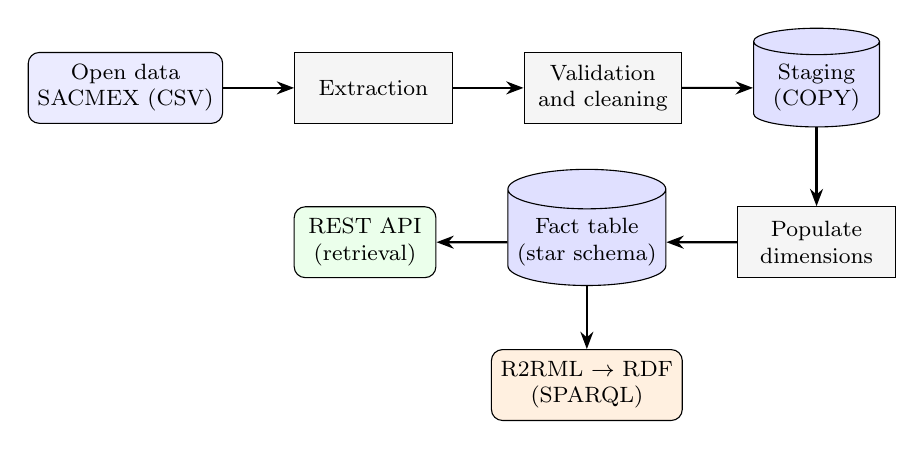
\begin{tikzpicture}[
    node distance=6mm and 9mm,
    font=\footnotesize,
    src/.style={draw, rounded corners, fill=blue!8, minimum height=9mm, minimum width=20mm, align=center},
    proc/.style={draw, fill=gray!8, minimum height=9mm, minimum width=20mm, align=center},
    store/.style={draw, cylinder, shape border rotate=90, aspect=0.25, fill=blue!12, minimum height=12mm, minimum width=16mm, align=center},
    endpt/.style={draw, rounded corners, fill=green!8, minimum height=9mm, minimum width=18mm, align=center},
    kg/.style={draw, rounded corners, fill=orange!12, minimum height=9mm, minimum width=18mm, align=center},
    flow/.style={-{Stealth[length=2.2mm]}, thick}
]
\node[src] (csv) {Open data\\SACMEX (CSV)};
\node[proc, right=of csv] (ext) {Extraction};
\node[proc, right=of ext] (val) {Validation\\and cleaning};
\node[store, right=of val] (stg) {Staging\\(COPY)};
\node[proc, below=10mm of stg] (dim) {Populate\\dimensions};
\node[store, left=of dim] (fact) {Fact table\\(star schema)};
\node[endpt, left=of fact] (api) {REST API\\(retrieval)};
\node[kg, below=8mm of fact] (kgn) {R2RML $\rightarrow$ RDF\\(SPARQL)};

\draw[flow] (csv) -- (ext);
\draw[flow] (ext) -- (val);
\draw[flow] (val) -- (stg);
\draw[flow] (stg) -- (dim);
\draw[flow] (dim) -- (fact);
\draw[flow] (fact) -- (api);
\draw[flow] (fact) -- (kgn);
\end{tikzpicture}%
}
\caption{ETL process architecture: from SACMEX heterogeneous open data to the
star schema exposed through a REST API \new{and, through a declarative R2RML
mapping, as an RDF knowledge graph}.}
\label{fig:etl}
\end{figure}

\subsection{Frontend and Geospatial Visualisation}

The frontend offers a dashboard with indicators, interactive charts (Plotly), and
a choropleth map of the 16 boroughs (Leaflet + GeoJSON), where colour represents
the consumption level and each borough displays a popup with its detail
(Fig.~\ref{fig:mapa}).

\begin{figure}[tbp]
\centering
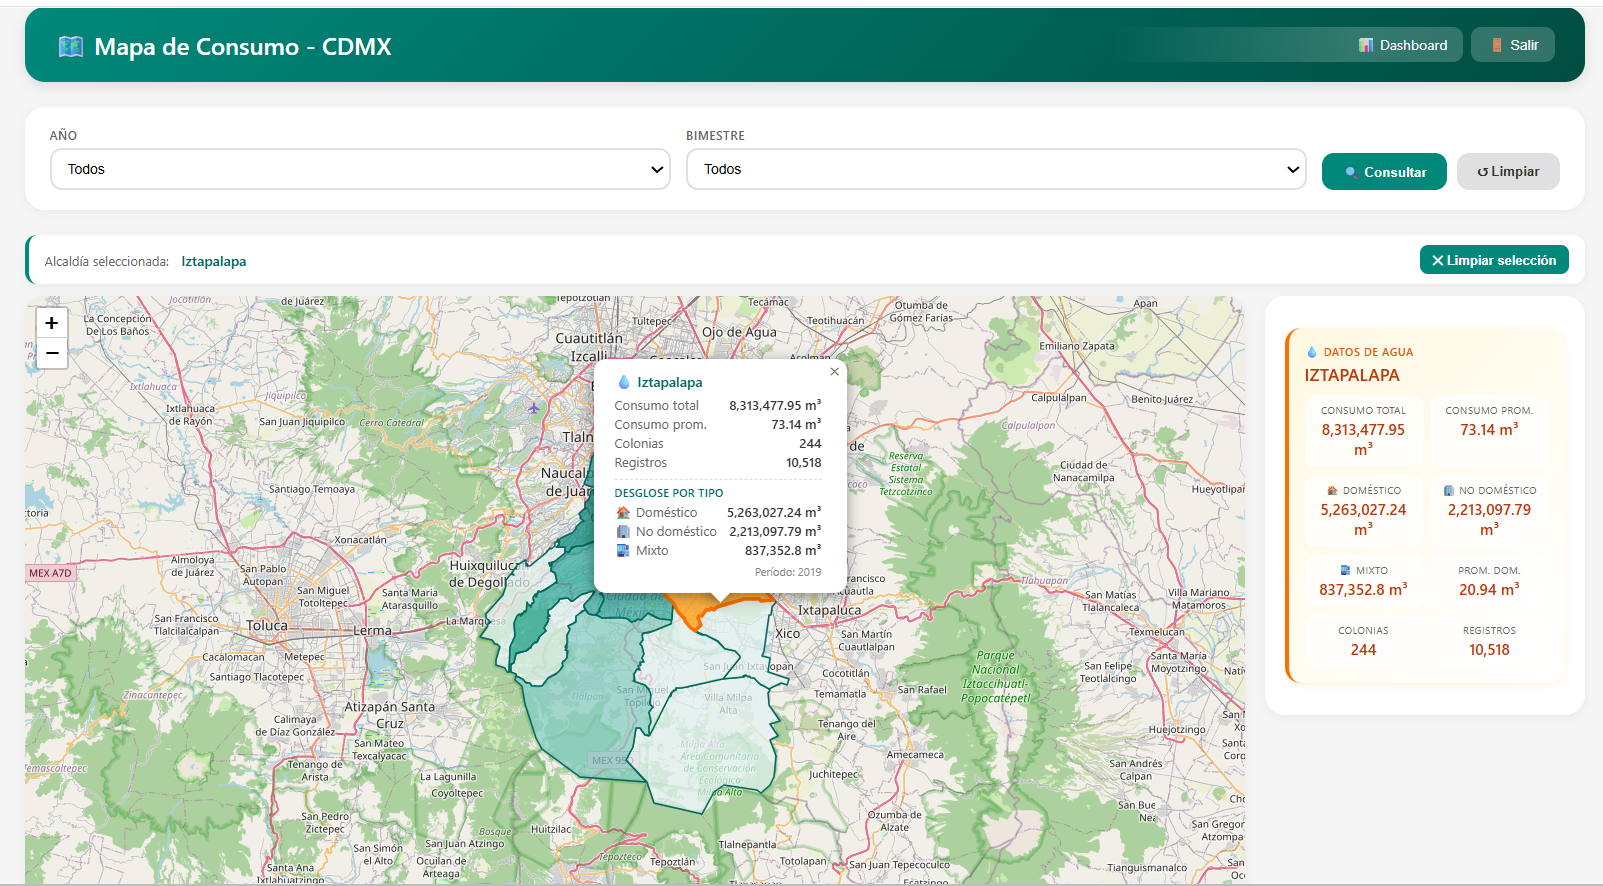
\includegraphics[width=0.78\linewidth,keepaspectratio]{Mapa.png}
\caption{Interactive map of water consumption by borough in Mexico City.}
\label{fig:mapa}
\end{figure}

\subsection{Implementation of the Atypical-Consumption Module}
\label{sec:atypical}

The current version replaces the idea of a traditional supervised prediction with
an atypical-consumption detection module oriented to analytical retrieval.
Instead of training a model with historical anomaly labels ---which are not
available in the open source--- the system computes statistical indicators over
the filtered records and detects zones whose consumption departs significantly
from the aggregate behaviour.

The procedure is implemented as an unsupervised analysis on the frontend: first,
the records are grouped by borough, neighbourhood, year, and bimester; then
reference measures such as total consumption, average consumption, and relative
dispersion are computed; finally, the zones with the largest deviation are
ordered to show them as possible atypical consumption. This approach avoids
presenting a prediction as if it were a model trained with reference data (ground
truth), but keeps the practical value of the analysis component by flagging
patterns that require later inspection.

Formally, for each territorial group $g$ an atypicality score $A_g$ is computed
from the normalised deviation with respect to the mean of the filtered set:
\begingroup
\setlength{\abovedisplayskip}{4pt}
\setlength{\belowdisplayskip}{4pt}
\begin{equation}
A_g = \left| \frac{x_g - \mu}{\sigma + \epsilon} \right| ,
\end{equation}
\endgroup
where $x_g$ represents the aggregate consumption of the group, $\mu$ is the
average consumption of comparable groups \new{---that is, of the groups that
remain after applying the same filter combination selected by the user, which
constitutes the reference population against which the deviation is measured---},
$\sigma$ is the standard deviation, and $\epsilon$ prevents division by zero. The
groups with the largest $A_g$ are reported in the interface as zones with
atypical consumption.

\begin{chgblock}
Two clarifications are necessary to delimit what this module does and does not
do. First, it is an \emph{exploratory anomaly-detection} component and not a
causal predictor of consumption: a high $A_g$ states that a zone departs from its
comparison set, not why. Second, and in direct response to a possible reading of
the results in Section~\ref{sec:mleval}, the module does \emph{not} perform
real-time leak detection. No real leak reports, no work orders and no network
telemetry are integrated into the warehouse, and the quantitative evaluation
reported below was obtained exclusively over synthetically injected
perturbations. Its operational role is to prioritise zones for later inspection
by the utility, which is a retrieval task ---ranking territorial units by a
computed score--- and not a diagnostic one.
\end{chgblock}

\subsection{Continuous Deployment Methodology}
\label{sec:deploy}

To guarantee that the demonstration remains available and reproducible without
depending on the availability of a server, the system is published in two
complementary modalities. The \textbf{dynamic deployment} keeps the complete
architecture ---FastAPI over PostgreSQL--- and serves parameterised queries and
aggregations against the data warehouse; it was used to obtain the experimental
results reported in this article, and its availability depends on the hosting
service. The \textbf{static version} exports the consolidated data as JSON and
GeoJSON files that the frontend consumes directly, so that querying, filtering,
aggregation and visualisation work on the client without an active backend. The
public repository is the preservation mechanism: it allows the static version to
be reconstructed and executed independently and indefinitely. \new{This duality addresses the recurring practical
problem that academic prototypes stop working shortly after evaluation, a concern
also raised by Hill et al.~\cite{hill2023}.}

The system is available at the following addresses:
\begin{itemize}\setlength{\itemsep}{1pt}
    \item \textbf{Public repository:} \new{\url{https://github.com/Uriel1024/Data_Warehouse_static}}
    \item \textbf{Static demo (permanent, no backend required):} \new{\url{https://uriel1024.github.io/Data_Warehouse_static/}}
\end{itemize}

The experimental results, the statistical analysis, and the findings reported in
this article were obtained over the original data warehouse built from the
official SACMEX open data, comprising 70,886 records. The static version is
intended to show the operation of the information-retrieval interface and does
not replace the database used for the experimental evaluation.


\subsection{Technologies Used}

The backend is implemented with FastAPI and Python~3.10 over Uvicorn; the
warehouse runs on PostgreSQL~14 accessed through psycopg2; the frontend uses
HTML5, CSS3, JavaScript, Leaflet and Plotly.js, consuming JSON and GeoJSON
exports; the ETL is written in Python and SQL; and \new{the graph layer relies
on an R2RML mapping targeting the RDF Data Cube and GeoSPARQL vocabularies,
queried with SPARQL~1.1}.

% =====================================================================
\begin{chgblock}
\section{From the Dimensional Model to a Knowledge Graph}
\label{sec:kg}

\subsection{Rationale: Why a Star Schema, and What a Graph Adds}

The choice of a relational star schema as the primary store was not made by
default, and it is worth justifying it explicitly. The dominant workload of the
system is the repeated aggregation of a single numeric measure over three
conformed dimensions ---time, territory and development level--- with filter
combinations chosen interactively by the user. This is precisely the workload for
which dimensional modelling was designed~\cite{kimball}: the star schema keeps
the join depth constant at one, allows the aggregate to be computed by a single
scan with grouping, and is directly supported by the indexing and query planning
of a mature relational engine. A graph representation of the same data would pay
a traversal cost for joins that the star schema resolves with foreign keys, and
would not, by itself, accelerate the aggregation.

What a graph representation adds is complementary rather than competing:
\emph{interoperability}, since a standard vocabulary makes the resource linkable
to other municipal datasets without prior schema agreement, the recurring
obstacle identified in the open-data
literature~\cite{quarati2023,nikiforova2021,weil2023};
\emph{topological expressiveness}, since questions such as ``which neighbourhoods
adjacent to a zone with atypical consumption also exceed the borough mean'' are
natural traversals over an adjacency relation and awkward over a flat territorial
dimension; and \emph{entity reconciliation}, since dereferenceable identifiers
aligned with external authorities resolve the label heterogeneity that our ETL
currently absorbs through normalisation rules. We therefore keep the star schema
as the analytical store and derive an RDF layer from it by a declarative mapping,
so that neither representation is maintained by hand.

\subsection{Vocabulary Alignment and R2RML Mapping}
\label{sec:mapping}

The correspondence between a star schema and the RDF Data Cube
vocabulary~\cite{datacube} is close to mechanical, which is what makes this layer
inexpensive to maintain. Table~\ref{tab:kg_mapping} states the alignment adopted.

\begin{table}[tbp]
\centering
\caption{Alignment between the dimensional model and the RDF vocabularies.}
\label{tab:kg_mapping}
{\ifshowchanges\color{chg}\fi
\footnotesize
\begin{tabularx}{\textwidth}{@{}lYY@{}}
\toprule
\textbf{Relational element} & \textbf{RDF construct} & \textbf{Vocabulary} \\
\midrule
\texttt{fact\_water\_consumption} (row) & \texttt{qb:Observation}        & RDF Data Cube \\
Measures (total, average, m$^3$)        & \texttt{qb:MeasureProperty}    & RDF Data Cube \\
\texttt{dim\_time}, \texttt{dim\_location} & \texttt{qb:DimensionProperty}  & RDF Data Cube \\
Borough / neighbourhood entity          & \texttt{geo:Feature}, \texttt{geo:asWKT} & GeoSPARQL \\
Territorial adjacency                   & \texttt{geo:sfTouches}         & GeoSPARQL \\
\texttt{dim\_dev\_index}                & \texttt{skos:Concept}          & SKOS \\
Billing category (dom./non-dom./mixed)  & \texttt{qb:AttributeProperty}  & RDF Data Cube \\
\bottomrule
\end{tabularx}
}
\end{table}

The mapping is expressed in R2RML~\cite{r2rml}, the W3C recommendation for
transforming relational content into RDF; RML~\cite{dimou2014} would allow the
same rules to be applied directly to the source CSV files, which is the variant
we intend to adopt when the pipeline is generalised to further open-data domains.
Listing~\ref{lst:r2rml} shows the triples map for the fact table; the complete
mapping is distributed with the repository.

\begin{lstlisting}[caption={Excerpt of the R2RML triples map for the fact table.},label={lst:r2rml}]
@prefix rr:   <http://www.w3.org/ns/r2rml#> .
@prefix qb:   <http://purl.org/linked-data/cube#> .
@prefix geo:  <http://www.opengis.net/ont/geosparql#> .
@prefix agua: <https://w3id.org/cdmx/agua/> .

<#ObservationMap> a rr:TriplesMap ;
  rr:logicalTable [ rr:tableName "fact_water_consumption" ] ;
  rr:subjectMap [ rr:template "https://w3id.org/cdmx/agua/obs/{fact_id}" ;
                  rr:class qb:Observation ] ;
  rr:predicateObjectMap [ rr:predicate qb:dataSet ;
                          rr:objectMap [ rr:constant agua:consumoCDMX ] ] ;
  rr:predicateObjectMap [ rr:predicate agua:location ;
                          rr:objectMap [ rr:parentTriplesMap <#LocationMap> ] ] ;
  rr:predicateObjectMap [ rr:predicate agua:totalConsumption ;
                          rr:objectMap [ rr:column "consumo_total" ;
                                         rr:datatype xsd:decimal ] ] .

<#LocationMap> a rr:TriplesMap ;
  rr:logicalTable [ rr:tableName "dim_location" ] ;
  rr:subjectMap [ rr:template "https://w3id.org/cdmx/agua/colonia/{location_id}" ;
                  rr:class geo:Feature ] ;
  rr:predicateObjectMap [ rr:predicate geo:asWKT ;
                          rr:objectMap [ rr:column "wkt" ;
                                         rr:datatype geo:wktLiteral ] ] .
\end{lstlisting}

\subsection{Territorial Retrieval as Graph Traversal}
\label{sec:sparql}

The value of the layer is that it makes a class of territorial questions
expressible that the tabular interface does not naturally support. GeoSPARQL~1.1
supplies the topological predicates~\cite{geosparql11,carhomburg2022}, and
current triple stores implement them at a level verified by the compliance
benchmark of Jovanovik et al.~\cite{jovanovik2021}. Listing~\ref{lst:sparql}
gives the query for the adjacency example discussed above: it retrieves the
neighbourhoods that border a zone flagged as atypical and whose own consumption
exceeds the borough mean, a pattern that would require either a materialised
adjacency table or a recursive query in the relational setting.

\begin{lstlisting}[caption={SPARQL query combining the statistical cube with the GeoSPARQL topology.},label={lst:sparql}]
PREFIX qb:   <http://purl.org/linked-data/cube#>
PREFIX geo:  <http://www.opengis.net/ont/geosparql#>
PREFIX agua: <https://w3id.org/cdmx/agua/>

SELECT ?neighbour (SUM(?m) AS ?total) WHERE {
  agua:colonia/flagged  geo:sfTouches  ?neighbour .
  ?obs  a qb:Observation ;
        agua:location ?neighbour ;
        agua:period   ?p ;
        agua:totalConsumption ?m .
  ?p    agua:bimester "2" .
}
GROUP BY ?neighbour
HAVING (SUM(?m) > 1739.40)
ORDER BY DESC(?total)
\end{lstlisting}

\subsection{Comparison of Candidate Data Models}

Table~\ref{tab:models} summarises the trade-off that motivated the hybrid design,
comparing the relational star schema, a labelled property graph, and an RDF
knowledge graph against the requirements of this use case.

\begin{table}[tbp]
\centering
\caption{Comparison of candidate data models for territorial retrieval of water
consumption.}
\label{tab:models}
{\ifshowchanges\color{chg}\fi
\footnotesize
\begin{tabularx}{\textwidth}{@{}lYYY@{}}
\toprule
\textbf{Requirement} & \textbf{Star schema} & \textbf{Property graph} & \textbf{RDF graph} \\
\midrule
Interactive aggregation over 10$^5$ rows & Very good & Moderate & Moderate \\
Multi-filter slicing (time, place, index) & Very good & Good & Good \\
Topological / adjacency queries & Weak (needs extra table) & Good & Very good (GeoSPARQL) \\
Linking to external datasets & Weak (schema agreement) & Moderate & Very good (IRIs) \\
Standard published vocabulary & No & No & Yes (Data Cube) \\
Schema evolution & Rigid & Flexible & Flexible \\
Operational cost for this prototype & Low & Medium & Medium \\
\bottomrule
\end{tabularx}
}
\end{table}

The conclusion, which we consider transferable to comparable municipal
open-data projects, is that the two models answer different questions and that
deriving the second from the first through a declarative mapping costs far less
than maintaining either alone. Materialising the full graph into a triple store
and comparing SPARQL against SQL over an equivalent workload are reported as
ongoing work in Section~\ref{sec:con}.
\end{chgblock}

% =====================================================================
\section{Results and Evaluation}
\label{sec:res}

\subsection{Integrated Data Volume}
\label{sec:volume}

The ETL process consolidated the water-consumption information of Mexico City
into the dimensional warehouse. Table~\ref{tab:volumen_datos} presents the stored
volume. The consistency of the reported volumes was verified directly on the
original data warehouse: the fact table contains 70,886 records, while the
dimensions contain 1,553 locations, 181 time records, and 4 development-index
levels. \new{As stated in Section~\ref{sec:met}, the 181 rows of
\texttt{dim\_time} correspond to distinct reading dates present in the source and
not to year--bimester combinations, and the 1,553 rows of \texttt{dim\_location}
are coarser than the fact grain.}

\begin{table}[tbp]
\centering
\caption{Data volume stored in the data warehouse.}
\label{tab:volumen_datos}
\begin{tabular}{@{}lr@{}}
\toprule
\textbf{Table} & \textbf{Records} \\
\midrule
\texttt{fact\_water\_consumption} & 70,886 \\
\texttt{dim\_location}            & 1,553 \\
\texttt{dim\_time}                & 181 \\
\texttt{dim\_dev\_index}          & 4 \\
\bottomrule
\end{tabular}
\end{table}

\subsection{Findings of the Consumption Analysis}
\label{sec:findings}

The analysis of the 70,886 consolidated records reveals the following consumption
patterns in Mexico City.

\textbf{Territorial concentration.} The boroughs with the highest total
consumption are Cuauht\'emoc and Miguel Hidalgo, followed by Benito Ju\'arez and
Gustavo A. Madero (Table~\ref{tab:top5_alcaldias}).
\new{This ordering requires a more careful reading than ``the boroughs that
consume the most''. Cuauht\'emoc, Miguel Hidalgo and Benito Ju\'arez concentrate
the historic centre and the densest commercial activity of the city, so their
totals aggregate a residential base with substantial non-domestic demand, whereas
Gustavo A. Madero and \'Alvaro Obreg\'on are among the most populous boroughs and
reach comparable totals through volume of households. The warehouse supports the
distinction directly, since the source separates domestic, non-domestic and mixed
billing: the non-domestic share is \fillin{\% Cuauht\'emoc} against
\fillin{\% Gustavo A. Madero}. Total consumption is therefore not a per-capita
indicator and should not be used as one for allocating supply interventions; the
per-account average, also stored in the warehouse, is the appropriate measure.}

\textbf{Temporal distribution.} Consumption shows variations across the
bimesters available in the warehouse. In the aggregated query by bimester, the
highest total consumption was observed in bimester~2, followed by bimester~3 and
bimester~1 (Table~\ref{tab:consumo_bimestre}). \new{The spread between the
extreme bimesters is below 10\,\% of the mean, and the warehouse covers only
three consecutive billing periods, which is insufficient to separate a seasonal
signal from ordinary billing variation.} Therefore, no direct causal relationship
with dry or rainy periods is established without integrating additional climatic
variables \new{and at least two complete annual cycles}.

\textbf{Relationship with the development index.} Neighbourhoods with a High
development index show a higher average consumption than those with a Low index.
\new{The index is published as part of the source dataset rather than derived by
us, and the portal does not document the methodology by which it was constructed;
this is an instance of the missing-metadata problem quantified by Vetr\`o et
al.~\cite{vetro2016} and by Quarati~\cite{quarati2023}. The observation is
therefore descriptive and internally consistent, but attributing it to a
socioeconomic mechanism would require an externally documented index, and we
report it as an association rather than as a causal relationship.}

\begin{table}[tbp]
\centering
\begin{minipage}[t]{0.52\textwidth}
\centering
\caption{Five boroughs with the highest total water consumption \new{(m$^3$,
aggregated over the three available bimesters)}.}
\label{tab:top5_alcaldias}
\footnotesize
\begin{tabular}{@{}lr@{}}
\toprule
\textbf{Borough} & \textbf{Total (m$^3$)} \\
\midrule
Cuauht\'emoc        & 18,401,765.79 \\
Miguel Hidalgo      & 14,490,397.15 \\
Benito Ju\'arez     & 13,780,118.64 \\
Gustavo A. Madero   & 13,480,100.57 \\
\'Alvaro Obreg\'on  &  9,608,545.20 \\
\bottomrule
\end{tabular}
\end{minipage}\hfill
\begin{minipage}[t]{0.44\textwidth}
\centering
\caption{Total and average consumption by bimester \new{(m$^3$; average per fact
record)}.}
\label{tab:consumo_bimestre}
\footnotesize
\begin{tabular}{@{}crr@{}}
\toprule
\textbf{Bim.} & \textbf{Avg.} & \textbf{Total} \\
\midrule
1 & 1,618.82 & 37,663,466.69 \\
2 & 1,739.40 & 41,519,580.96 \\
3 & 1,733.65 & 41,174,097.68 \\
\bottomrule
\end{tabular}
\end{minipage}
\end{table}

The interface dynamically generates the list of neighbourhoods with the highest
total consumption according to the filters selected by the user, so that the
analytical outputs of the system ---top neighbourhoods, total consumption by
borough, average consumption per record, and the atypical-consumption ranking---
are always relative to the active query rather than fixed in advance.

\subsection{The Atypical-Consumption Module within the Retrieval Framework}

The atypical-consumption module makes it possible to order boroughs or
neighbourhoods according to their deviation from the average behaviour of the
filtered set. \new{Its role within the overall framework is best understood as a
ranking function rather than as an analytical add-on. The choropleth map answers
``how much is consumed here''; the module answers ``which territorial units
should I look at first'', which is the ordering problem at the centre of
information retrieval~\cite{purves2018}. It consumes the same filtered result set
that the retrieval interface produces, and returns a permutation of it, so that
the user moves from browsing to a prioritised list without changing the query.
This is what turns a descriptive visualisation into an exploration tool: the
score is not a diagnosis, it is a relevance criterion for territorial units.}

\subsection{Quantitative Evaluation of the Atypical-Consumption Module}
\label{sec:mleval}

Although the module operates in an unsupervised manner in production ---the open
source provides no anomaly labels--- its performance was evaluated through a
controlled and reproducible protocol with injected anomalies acting as ground
truth. Over a synthetic set with the structure of the warehouse
($N\approx11{,}460$ records from 16 boroughs), 3\,\% of labelled anomalies were
injected (70\,\% high spikes, 30\,\% drops) and three detectors were compared:
the $A_g$ z-score of this work, Isolation Forest, and LOF, using as features the
log-scaled consumption and its ratio to the neighbourhood mean.
Table~\ref{tab:eval_ml} reports precision, recall, F1, and the areas under the
ROC and precision--recall curves.

\begin{table}[tbp]
\centering
\caption{Evaluation of the atypical-consumption detection module on injected
anomalies (synthetic ground truth; $N\approx11{,}460$, 3\,\% anomalies, fixed
seed). Reproducible with \texttt{evaluacion-ml/eval\_anomalias.py}.}
\label{tab:eval_ml}
\footnotesize
\begin{tabular}{@{}lccccc@{}}
\toprule
\textbf{Method} & \textbf{Precision} & \textbf{Recall} & \textbf{F1} & \textbf{ROC-AUC} & \textbf{PR-AUC} \\
\midrule
z-score $A_g$ (this work) & 1.000 & 0.497 & 0.664 & 0.987 & 0.816 \\
Isolation Forest          & 0.940 & 1.000 & 0.969 & 1.000 & 1.000 \\
LOF                       & 0.135 & 0.029 & 0.048 & 0.555 & 0.062 \\
\bottomrule
\end{tabular}
\end{table}

The z-score reaches perfect precision but moderate recall (0.50): it reliably
detects extreme spikes, although its fixed threshold misses part of the drops.
\new{The asymmetry follows from the shape of the data rather than from the
statistic itself: consumption is bounded below by zero, so an injected drop
produces a smaller absolute deviation than an injected spike of the same relative
magnitude, and a symmetric threshold at $A_g>3$ therefore captures the spikes
while leaving part of the drops below the cut.} Isolation Forest offers the best
trade-off (F1 $=0.97$), while LOF proves poorly suited to this type of
global-magnitude anomaly (F1 $=0.05$). These results support the use of the
z-score as a high-precision exploratory filter and point to Isolation Forest as
the natural improvement of the module.

\textbf{Validity of the protocol.} These metrics do not represent performance
against real leaks or observed anomalies, but rather the ability of each method
to recover injected synthetic anomalies under a controlled protocol. This
decision is due to the fact that the open source does not provide real anomaly
labels. \new{Three limitations of the protocol must be stated. First, the
features used ---log-scaled consumption and ratio to the neighbourhood mean---
are aligned with the mechanism by which the anomalies were injected, which
inflates the separability of the problem and explains the perfect areas under the
curve obtained by Isolation Forest; the figures should be read as an upper bound,
not as expected field performance. Second, the thresholds were not equalised
across methods: the z-score used the fixed statistical criterion $A_g>3$, while
Isolation Forest used $s>0.60$ and LOF $s>1.5$, so the comparison at a single
operating point favours the methods whose threshold was chosen. Third, and as
stated in Section~\ref{sec:atypical}, none of this constitutes evidence about
real-time leak detection, for which the system is not designed and for which no
labelled data were available.} Therefore, the results should be interpreted as a
reproducible evaluation of sensitivity to known perturbations, not as a
definitive operational validation.

\subsection{Performance Metrics}
\label{sec:perf}

The performance of the main dashboard was evaluated using Lighthouse (v13.2.0).
\new{The measurement was taken against the dynamic deployment serving the
complete warehouse, with the dashboard performing its initial render and its
first aggregate request; the client-side aggregation of the exported dataset in
the static version was measured separately and is not mixed into these figures.}
Table~\ref{tab:lighthouse_dashboard} summarises the metrics obtained.

\begin{table}[tbp]
\centering
\caption{Dashboard performance metrics (Lighthouse v13.2.0).}
\label{tab:lighthouse_dashboard}
\begin{tabular}{@{}lll@{}}
\toprule
\textbf{Metric} & \textbf{Value} & \textbf{Assessment} \\
\midrule
First Contentful Paint (FCP)   & 0.8 s & Excellent \\
Largest Contentful Paint (LCP) & 1.2 s & Good \\
Speed Index                    & 1.5 s & Excellent \\
Total Blocking Time (TBT)      & 0 ms  & Excellent \\
Cumulative Layout Shift (CLS)  & 0     & Excellent \\
\bottomrule
\end{tabular}
\end{table}

\begin{chgblock}
\textbf{Query execution over the total data volume.} Frontend metrics do not
characterise the retrieval layer, so the response time of the analytical
endpoints was measured directly against the warehouse. Three workloads were
distinguished: a paginated retrieval that returns a bounded page of facts, a
full-scan aggregation by borough that touches all 70,886 rows, and a full-scan
aggregation by neighbourhood and bimester, which is the heaviest query the
dashboard issues. Each workload was executed \fillin{n} times after a warm-up
round, on \fillin{hardware/hosting description}, with the results reported in
Table~\ref{tab:api_perf}. Reporting the 95th percentile over a sample of this
size, rather than over the ten executions of a single endpoint used in the
submitted version, is what makes the percentile meaningful.
\end{chgblock}

\begin{table}[tbp]
\centering
\caption{\new{Response time of the retrieval endpoints over the complete
warehouse (70,886 fact rows).}}
\label{tab:api_perf}
{\ifshowchanges\color{chg}\fi
\footnotesize
\begin{tabularx}{\textwidth}{@{}Yrrrr@{}}
\toprule
\textbf{Workload} & \textbf{Rows scanned} & \textbf{Mean (ms)} & \textbf{p95 (ms)} & \textbf{Executions} \\
\midrule
Paginated retrieval (\texttt{limit{=}100}) & 100 & 24.9 & 43.6 & 10 \\
Full aggregation by borough & 70,886 & \fillin{?} & \fillin{?} & \fillin{?} \\
Aggregation by neighbourhood and bimester & 70,886 & \fillin{?} & \fillin{?} & \fillin{?} \\
Top-10 neighbourhoods with ordering & 70,886 & \fillin{?} & \fillin{?} & \fillin{?} \\
\bottomrule
\end{tabularx}
}
\end{table}

\subsection{Functional Tests and Retrieval Capability}

The operation of the ETL processes, the persistence in PostgreSQL, the FastAPI
endpoints, and the information retrieval was verified. The tests included queries
parameterised by year, bimester, borough, and neighbourhood; aggregated retrieval
(total and average consumption by neighbourhood); generation of JSON responses;
geospatial retrieval for visualisation; and pagination with configurable limits.
All modules produced results consistent with the expected structure.
The dimensional model thus allows retrieving territorial information through
combined filters of time, location, and development index, executing analytical
queries over 70,886 records without directly accessing the original sources.

% =====================================================================
\begin{chgblock}
\section{Discussion}
\label{sec:disc}

\subsection{Comparison with Previous Systems}

Placed against the systems summarised in Table~\ref{tab:comparison}, the
contribution of this work is neither the dimensional model nor the dashboard,
both of which are well-established techniques, but the combination of an input
that the water-management literature has largely avoided with an output that the
open-data literature has repeatedly asked for. The water data warehouses of
Soares et al.~\cite{soares2019} and Duque-M\'endez et al.~\cite{duque2014} obtain
higher-quality input than ours ---meter readings and instrumented series--- at
the cost of depending on the utility's internal systems, which makes them
non-replicable by third parties and non-auditable by citizens. Abecker et
al.~\cite{abecker2014} anticipate our hybrid relational/RDF arrangement, but
again over proprietary sensor networks. Conversely, the urban knowledge graphs of
Liu et al.~\cite{liu2023} and Wang et al.~\cite{wang2023} operate on open input
and publish reusable artefacts, but target prediction and risk assessment rather
than the retrieval of billed consumption at territorial granularity.

The position we occupy is therefore the intersection: official open data as the
only input, a dimensional model for the aggregation workload, a standard graph
vocabulary for interoperability, and a permanently reachable demonstration. The
closest precedent on the last axis is Hill et al.~\cite{hill2023}, whose
wastewater-surveillance dashboard shares our concern with survivability, and
whose experience motivated our decision to export a self-contained static version
rather than to rely on a hosted backend.

\subsection{Practical Implications}

Three implications follow from the results. For the utility, the ranking produced
by the atypical-consumption module is a prioritisation aid whose value lies in
reducing the search space for inspection, not in diagnosing causes; used together
with the domestic / non-domestic decomposition of Section~\ref{sec:findings}, it
separates zones whose deviation is plausibly commercial from those where a
residential anomaly warrants a visit. For urban research, the consolidated
warehouse removes the preprocessing barrier that currently makes this dataset
expensive to use, and the graph layer of Section~\ref{sec:kg} lowers the cost of
joining it with other municipal sources. For open-data policy, the exercise is a
concrete measurement of the gap identified by
Quarati~\cite{quarati2023} and Nikiforova and McBride~\cite{nikiforova2021}: the
data were public throughout, yet a non-trivial engineering effort was required
before a citizen could answer a question as simple as how much water is billed in
their neighbourhood.

\subsection{Threats to Validity and Limitations}
\label{sec:limits}

Several limitations delimit the scope of the conclusions. The most consequential
concerns temporal coverage: the warehouse holds three consecutive billing
periods, which supports territorial comparison but not seasonal or trend
analysis, and any reading of the bimester differences as a seasonal effect would
be unwarranted. A second limitation concerns the development index, which is
consumed as published and whose construction methodology is not documented by the
source, so the association reported in Section~\ref{sec:findings} cannot be
promoted to a socioeconomic explanation. A third concerns the evaluation of the
detection module, which rests on synthetic perturbations whose feature signature
is aligned with the detectors, and which therefore establishes sensitivity to
known deviations rather than field performance against real leaks. A fourth
concerns the published static version, which serves exported JSON and GeoJSON
files and consequently does not execute SQL against the warehouse in real time;
the analytical results reported here were obtained on the dynamic deployment. A
fifth concerns the graph layer, which is delivered as a declarative mapping and a
set of example queries rather than as a materialised and benchmarked triple
store. Finally, the quality of the whole rests on the quality, coverage and
freshness of the source dataset, whose update cadence is outside our control and
whose metadata gaps we absorb but cannot repair.
\end{chgblock}

% =====================================================================
\section{Conclusions and Future Work}
\label{sec:con}

\subsection{Conclusions}

A data warehouse was presented for the territorial information retrieval of water
consumption in Mexico City, built from open sources through a reproducible ETL
process and published with a continuous-deployment methodology that guarantees a
permanent functional demonstration. The solution consolidated 70,886 consumption
records and 1,553 locations across the 16 boroughs into a dimensional star schema
on PostgreSQL. \new{On top of that schema, a declarative R2RML mapping aligned
with the RDF Data Cube and GeoSPARQL vocabularies republishes the same facts as a
knowledge graph, so that territorial retrieval can be expressed both as
relational aggregation and as topological traversal without duplicating the
maintenance effort.}

The findings reveal that water consumption in Mexico City is concentrated in the
boroughs of Cuauht\'emoc and Miguel Hidalgo (Table~\ref{tab:top5_alcaldias}), a
concentration that the domestic / non-domestic decomposition attributes to
commercial intensity rather than to residential demand alone, and that it varies
across the available bimesters by a margin too small, and over a window too
short, to support a seasonal interpretation. These results show that the system
not only consolidates data, but also allows extracting knowledge useful for water
management, while making explicit the boundary beyond which the available data do
not license further inference.

\new{The three central contributions ---the consolidation ETL, the graph layer
derived from the dimensional model, and the always-accessible demo
methodology--- constitute a replicable method for bringing heterogeneous official
open data to queryable, linkable and verifiable territorial information.}

\subsection{Future Work}

\new{The most immediate line of work is the materialisation of the knowledge
graph described in Section~\ref{sec:kg} into a triple store, together with a
quantitative comparison of SPARQL and SQL response times over an equivalent
workload and the reconciliation of borough and neighbourhood entities against
external authorities, which would place the resource in the Linked Open Data
cloud and allow it to be joined with other municipal datasets without prior
schema agreement. In parallel, the temporal coverage of the warehouse must be
extended to at least two complete annual cycles before any seasonal analysis is
attempted, and climatic variables integrated if the relationship with dry and
rainy periods is to be tested rather than merely observed.}

\new{The evaluation of the atypical-consumption module will be recomputed when
real labelled anomaly or leak data become available, reporting complete
precision--recall curves and a threshold sensitivity analysis at equalised
operating points, and replacing the current synthetic protocol whose optimism we
have made explicit. Finally, the method is domain-agnostic by construction, and
we intend to transfer it to other open urban-data domains ---mobility, air
quality and seismic risk--- where the same combination of dispersed official
files and absent query tooling recurs.}

% =====================================================================
\begin{chgblock}
\section*{Declaration on the Use of Generative AI}

The authors used a generative AI assistant as a writing and reviewing aid,
limited to language editing of the English text, formatting of the
\LaTeX{} source, and suggestions for restructuring the argument in response to
the reviewers' comments. The system design, the ETL implementation, the data
processing, the experiments and their interpretation were carried out by the
authors, who take full responsibility for the content of the article, verified
every cited reference against its original source, and confirm that no text was
reproduced from third-party works.
\end{chgblock}

\section*{Disclosure of Interests}

The authors declare that they have no conflicts of interest relevant to the
content of this article.

% =====================================================================
\begin{thebibliography}{99}

\bibitem{kimball} Kimball, R., Ross, M.: The Data Warehouse Toolkit: The Definitive Guide to Dimensional Modeling. 3rd edn. Wiley, Indianapolis (2013)

\bibitem{vassiliadis2009} Vassiliadis, P.: A survey of Extract--Transform--Load technology. International Journal of Data Warehousing and Mining \textbf{5}(3), 1--27 (2009). \url{https://doi.org/10.4018/jdwm.2009070101}

\bibitem{soares2019} Soares, J., Leite, P., Teixeira, P., Lopes, N., Silva, J.P.: Data warehouse for the monitoring and analysis of water supply and consumption. In: Ramos, I., Quaresma, R., Resende da Silva, P., Oliveira, T. (eds.) Information Systems for Industry 4.0. Springer, Cham (2019). \url{https://doi.org/10.1007/978-3-030-14850-8_1}

\bibitem{duque2014} Duque-M\'endez, N.D., Orozco-Alzate, M., V\'elez, J.J.: Hydro-meteorological data analysis using OLAP techniques. DYNA \textbf{81}(185), 168--175 (2014)

\bibitem{abecker2014} Abecker, A., Brauer, T., Magoutas, B., Mentzas, G., Papageorgiou, N., Quenzer, M.: A sensor and semantic data warehouse for integrated water resource management. In: EnviroInfo 2014. BIS-Verlag, Oldenburg (2014)

\bibitem{vetro2016} Vetr\`o, A., Canova, L., Torchiano, M., Orozco Minotas, C., Iemma, R., Morando, F.: Open data quality measurement framework. Government Information Quarterly \textbf{33}(2), 325--337 (2016). \url{https://doi.org/10.1016/j.giq.2016.02.001}

\bibitem{berro2015} Berro, A., Megdiche, I., Teste, O.: A content-driven ETL processes for open data. In: Bassiliades, N., et al. (eds.) New Trends in Database and Information Systems II. Springer, Cham (2015). \url{https://doi.org/10.1007/978-3-319-10518-5_3}

\bibitem{purves2018} Purves, R.S., Clough, P., Jones, C.B., Hall, M.H., Murdock, V.: Geographic information retrieval. Foundations and Trends in Information Retrieval \textbf{12}(2--3), 164--318 (2018). \url{https://doi.org/10.1561/1500000034}

\bibitem{han2019} Han, S.Y., Rey, S., Knaap, E., Kang, W., Wolf, L.: Adaptive Choropleth Mapper. ISPRS International Journal of Geo-Information \textbf{8}(11), 509 (2019). \url{https://doi.org/10.3390/ijgi8110509}

\bibitem{sandve2013} Sandve, G.K., Nekrutenko, A., Taylor, J., Hovig, E.: Ten simple rules for reproducible computational research. PLoS Computational Biology \textbf{9}(10), e1003285 (2013). \url{https://doi.org/10.1371/journal.pcbi.1003285}

\bibitem{hill2023} Hill, D., Dunham, C., Larsen, D.A., Collins, M.: Operationalizing an open-source dashboard for wastewater-based surveillance. MethodsX \textbf{11}, 102299 (2023). \url{https://doi.org/10.1016/j.mex.2023.102299}

\bibitem{villa2026} \fillin{restore the authors' own previous reference (seismic-risk data warehouse), withheld during review}

\bibitem{sacmex} SACMEX: Consumo de agua. Portal de Datos Abiertos de la Ciudad de M\'exico, Agencia Digital de Innovaci\'on P\'ublica. \url{https://datos.cdmx.gob.mx/dataset/consumo-agua}. \new{Accessed \fillin{date of download}}

\bibitem{quarati2023} Quarati, A.: Open government data: usage trends and metadata quality. Journal of Information Science \textbf{49}(4), 887--910 (2023). \url{https://doi.org/10.1177/01655515211027775}

\bibitem{nikiforova2021} Nikiforova, A., McBride, K.: Open government data portal usability: a user-centred usability analysis of 41 open government data portals. Telematics and Informatics \textbf{58}, 101539 (2021). \url{https://doi.org/10.1016/j.tele.2020.101539}

\bibitem{weil2023} Weil, C., Bibri, S.E., Longchamp, R., Golay, F., Alahi, A.: Urban digital twin challenges: a systematic review and perspectives for sustainable smart cities. Sustainable Cities and Society \textbf{99}, 104862 (2023). \url{https://doi.org/10.1016/j.scs.2023.104862}

\bibitem{carhomburg2022} Car, N.J., Homburg, T.: GeoSPARQL 1.1: motivations, details and applications of the decadal update to the most important geospatial LOD standard. ISPRS International Journal of Geo-Information \textbf{11}(2), 117 (2022). \url{https://doi.org/10.3390/ijgi11020117}

\bibitem{jovanovik2021} Jovanovik, M., Homburg, T., Spasi\'c, M.: A GeoSPARQL compliance benchmark. ISPRS International Journal of Geo-Information \textbf{10}(7), 487 (2021). \url{https://doi.org/10.3390/ijgi10070487}

\bibitem{geosparql11} Open Geospatial Consortium: OGC GeoSPARQL --- a geographic query language for RDF data, version 1.1. OGC Implementation Standard (2024)

\bibitem{datacube} World Wide Web Consortium: The RDF Data Cube vocabulary. W3C Recommendation, 16 January 2014. \url{https://www.w3.org/TR/vocab-data-cube/}

\bibitem{r2rml} World Wide Web Consortium: R2RML --- RDB to RDF mapping language. W3C Recommendation, 27 September 2012. \url{https://www.w3.org/TR/r2rml/}

\bibitem{dimou2014} Dimou, A., Vander Sande, M., Colpaert, P., Verborgh, R., Mannens, E., Van de Walle, R.: RML: a generic language for integrated RDF mappings of heterogeneous data. In: Workshop on Linked Data on the Web (LDOW 2014). CEUR Workshop Proceedings, vol. 1184 (2014)

\bibitem{dsouza2021} Dsouza, A., Tempelmeier, N., Yu, R., Gottschalk, S., Demidova, E.: WorldKG: a world-scale geographic knowledge graph. In: Proceedings of the 30th ACM International Conference on Information and Knowledge Management (CIKM), pp. 4475--4484. ACM (2021)

\bibitem{liu2023} Liu, Y., Ding, J., Fu, Y., Li, Y.: UrbanKG: an urban knowledge graph system. ACM Transactions on Intelligent Systems and Technology \textbf{14}(4), art.\ 60 (2023)

\bibitem{wang2023} Wang, Y., Ye, F., Li, B., Jin, G., Xu, D., Li, F.: UrbanFloodKG: an urban flood knowledge graph system for risk assessment. In: Proceedings of the 32nd ACM International Conference on Information and Knowledge Management (CIKM), pp. 2574--2584. ACM (2023)

\bibitem{roussey2023} Roussey, C., Gu\'eret, C., Laporte, M.-A.: Editorial: knowledge graph technologies --- the next frontier of the food, agriculture, and water domains. Frontiers in Artificial Intelligence \textbf{6}, 1319844 (2023). \url{https://doi.org/10.3389/frai.2023.1319844}

\bibitem{papageorgiou2025} Papageorgiou, N., Pournara, D., Apostolou, D., Mentzas, G.: Managing industrial water treatment processes knowledge with knowledge graphs. Web Intelligence (2025). \url{https://doi.org/10.1177/18724981251321368}

\bibitem{ramonell2023} Ramonell, C., Chac\'on, R., Posada, H.: Knowledge graph-based data integration system for digital twins of built assets. Automation in Construction \textbf{156}, 105109 (2023). \url{https://doi.org/10.1016/j.autcon.2023.105109}

\end{thebibliography}

\end{document}
